\documentclass[pscyr, 12pt]{hedlab}
\usepackage[russian]{babel}
\usepackage{graphicx}

\graphicspath{{images/}}

\labname{Разработка баз данных в СУБД Oracle}
\labnum{7}
\student{Голубев~А.~В., САПР-1.1п}
\labdate{}

\begin{document}
    \makeheader
    \noindent\textbf{Цель:} создание отчёта с параметрами

    \noindent\textbf{Постановка задачи:}\vspace*{-0.5em}
    \begin{itemize}\itemsep-5pt
        \item изучить функциональные возможности программы
        \item создать табличный отчёт с параметрами
        \item вывести данные на экран
    \end{itemize}

    Формируем запрос пользовательского параметра \emph{P\_MIN} делающий выборку по окладу
    \begin{figure}[ht!]
        \center
        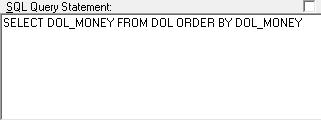
\includegraphics[width=0.47\textwidth]{lab07_01}
    \end{figure}

    Формируем SQL-запрос c использованием пользовательского параметра 
    \begin{figure}[ht!]
        \center
        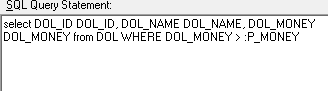
\includegraphics[width=0.47\textwidth]{lab07_02}
    \end{figure}

    Формируем форму для выбора значения параметра
    \begin{figure}[ht!]
        \center
        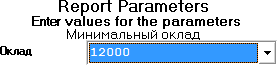
\includegraphics[width=0.47\textwidth]{lab07_03}
    \end{figure}

    Результат выборки из БД по пользовательскому параметру
    \begin{figure}[ht!]
        \center
        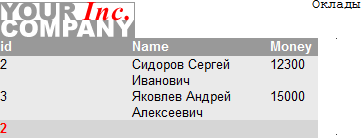
\includegraphics[width=0.47\textwidth]{lab07_04}
    \end{figure}

    \noindent\textbf{Вывод:} в результате проделанной работы\vspace*{-0.5em}
    \begin{enumerate}\itemsep-5pt
        \item создан отчёт по таблице из БД
        \item создан пользовательский параметр делающий выборку по окладу
        \item изучен базовый функционал программы формирования отчётов
    \end{enumerate}
\end{document}